%%%%%%%% ICML 2018 EXAMPLE LATEX SUBMISSION FILE %%%%%%%%%%%%%%%%%

\documentclass{article}

% Recommended, but optional, packages for figures and better typesetting:
\usepackage{microtype}
\usepackage{graphicx}
\usepackage{subfigure}
\usepackage{booktabs} % for professional tables
\usepackage{url}
\usepackage{cite}
\usepackage{subfigure}
\usepackage{amsmath} 
\usepackage{amsfonts}
\usepackage{amssymb,bm}
 

% hyperref makes hyperlinks in the resulting PDF.
% If your build breaks (sometimes temporarily if a hyperlink spans a page)
% please comment out the following usepackage line and replace
% \usepackage{icml2018} with \usepackage[nohyperref]{icml2018} above.
\usepackage{hyperref}
\usepackage{breakurl}
\hypersetup{breaklinks=true} % set automatically by hyperref?

% Attempt to make hyperref and algorithmic work together better:
\newcommand{\theHalgorithm}{\arabic{algorithm}}

% Use the following line for the initial blind version submitted for review:
% \usepackage{icml2018}

% If accepted, instead use the following line for the camera-ready submission:
\usepackage[accepted]{icml2018}

% The \icmltitle you define below is probably too long as a header.
% Therefore, a short form for the running title is supplied here:
%\icmltitlerunning{Submission and Formatting Instructions for ICML 2018}

\begin{document}

\twocolumn[
\icmltitle{Meta-learning for image/video classification}

% It is OKAY to include author information, even for blind
% submissions: the style file will automatically remove it for you
% unless you've provided the [accepted] option to the icml2018
% package.

% List of affiliations: The first argument should be a (short)
% identifier you will use later to specify author affiliations
% Academic affiliations should list Department, University, City, Region, Country
% Industry affiliations should list Company, City, Region, Country

% You can specify symbols, otherwise they are numbered in order.
% Ideally, you should not use this facility. Affiliations will be numbered
% in order of appearance and this is the preferred way.
\icmlsetsymbol{equal}{*}

\begin{icmlauthorlist}
\icmlauthor{Philipp Jankov}{}
\icmlauthor{Christopher Krolla}{}
\icmlauthor{Thomas Nierhoff}{}
\end{icmlauthorlist}

%\icmlaffiliation{fr}{University of Freiburg, Freiburg, Germany}

\icmlcorrespondingauthor{Philipp Jankov}{philipp.jankov@gmail.com}
\icmlcorrespondingauthor{Christopher Krolla}{krollac.ck@gmail.com}
\icmlcorrespondingauthor{Thomas Nierhoff}{thomasnierhoff@web.de}

% You may provide any keywords that you
% find helpful for describing your paper; these are used to populate
% the "keywords" metadata in the PDF but will not be shown in the document
\icmlkeywords{Machine Learning, Freiburg}

\vskip 0.3in
]

% this must go after the closing bracket ] following \twocolumn[ ...

% This command actually creates the footnote in the first column
% listing the affiliations and the copyright notice.
% The command takes one argument, which is text to display at the start of the footnote.
% The \icmlEqualContribution command is standard text for equal contribution.
% Remove it (just {}) if you do not need this facility.

%\printAffiliationsAndNotice{}  % leave blank if no need to mention equal contribution
%\printAffiliationsAndNotice{\icmlEqualContribution} % otherwise use the standard text.


%%%%%%%%%%%%%%%%%%%%%%%%%%%%%%%%%%%%%%%%%%%%%%%%%%%%%%%%%%%%%%%%%%%%%%%%%%%%%%%%
\begin{abstract}
This documentation summarizes the progress of the automl{\textunderscore}freiburg video team on the AutoDL $2019-2020$ challenge. Two methods are presented: The first method relies on transfer learning of a single, pretrained video classification network which is fine tuned during the challenge. As this approach has shown several limitations if the test datasets vary too much, a more elaborate method based on meta learning is developed: Multiple classification networks are evaluated on different training datasets a priori and the incumbent for every dataset is stored in a lookup table. During test time, the similarity between the test dataset and all training datasets is measured and the incumbent of the most similar training dataset is used for training/evaluation on the test dataset. The first method has been submitted and evaluated on the AutoCV2 challenge and resulted in a mediocre score. Four different approaches are presented and evaluated for the second method, resulting in scores almost on par with the best performing image and video classification team.
\end{abstract}




%%%%%%%%%%%%%%%%%%%%%%%%%%%%%%%%%%%%%%%%%%%%%%%%%%%%%%%%%%%%%%%%%%%%%%%%%%%%%%%%
\section{Introduction}
Machine learning (ML) based on artificial neural networks is a fast-growing field in the domain of computer science. Instead of manually tweaking the features used for classification or regression, neural networks are able to extract them automatically. They have shown state-of-the-art performance on a variety of classification problems when trained on huge datasets and are well suited for parallelization. 

A open question is how to deal with computational limitations and generic datasets. In many real-world applications (e.g. smartphones) computational resources, execution time and storage capacity is limited. Thus the current trend of using larger and larger networks for better classification results becomes unfeasible. In addition, it may be not known a priori what the data to be classified looks like, requiring the neural network to be applicable to a variety of different datasets. Multiple approaches emerged within the last years to tackle both challenges:

To reduce the model size (and thus implicitly also execution time, storage capacity and computational resources), one can remove the most ``unimportant'' parts of a neural network and/or quantize it, resulting in a compression of the neural network The selection of the nodes/layers to be pruned can either be specified manually or derived automatically through reinforcement learning~\cite{han15,han18}. A second option is knowledge distillation where a smaller student``network'' is trained to produce outputs similar to a previously trained larger ``teacher'' network~\cite{hinton14,phuong19}. By using the logits output instead of the softmax output, much more information is preserved in every training step. Consequently training the student network can be achieved with less samples. For both approaches there is only a negligible decrease in classification accuracy while the compression rate can be huge (up to a factor of 496x for certain layers of a neural network ~\cite{reagan18}). Another more straightforward method is to search directly for smaller/faster models. This can be either done manually - see e.g.~\cite{howard17} - or through neural architecture search~\cite{elsken19}. Note that the last approach can output networks that are state of the art with respect to model size, speed and classification accuracy~\cite{tan19}.

Other techniques are used if the time budget for training is tight or the dataset to be trained on is not known a priori. They all have in common that a network is pretrained on one or more datasets and information from pretraining is subsequently used for the final training step. One technique is transfer learning~\cite{pan10}. Here the common use case consists of pretraining a network on a large dataset to initialize the network weights with reasonable values. If a new dataset is similar enough, only parts of the network (e.g. the last layers of a convolutional neural network) must be trained again. In addition, the new dataset can be rather small as less optimization steps are required (the network is not trained from scratch). Another option is meta learning or learning to learn~\cite{santoro16,hutter19}: By learning multiple models for multiple tasks (or more specific: datasets) beforehand, it is quite likely that a new task will be similar to a previously learned task. In this case, knowledge gained from the previous task can be reused, thus accelerating the learning progress. The challenge with meta learning is a proper selection of the meta features to be extracted as their predictive capabilities vary heavily~\cite{bilalli17}. One predominant meta learning approach at the moment is MAML \cite{finn17}, optimizing a model not for classification accuracy but specifically for good generalization to unseen datasets from the same dataset distribution. 

The AutoDL challenge contains both aspects, tight computational limitations (both time- and resource-wise) and generic datasets. As such it provides an ideal testbed for advanced approaches in order to find time-efficient algorithms with a small memory footprint. Because the datasets are undisclosed, the options for manual tweaking are limited. Instead of highly specific solutions tied to a specific environment one is thus seeking for a fast yet robust approach. This makes the challenge different from ``traditional'' benchmarks like ImageNet classification where computing power is solely limited by the budget of the chair/institute and the dataset is known beforehand.

The remainder of the paper is organized as follows: Section~\ref{sec:autodl} and section~\ref{sec:datasets} provide general background information about the AutoDL challenge and an overview of the used datasets. A first method used during the AutoCV2 video challenge is presented in section~\ref{sec:tl}. As focus shifted after the video challenge, section~\ref{sec:ml} illustrates two more elaborate approaches for video and image classification that can be used for the final AutoDL challenge. The do\-cumentation concludes with a short discussion in section~\ref{sec:discussion} and a summary with possible future directions in section~\ref{sec:summary}.


%%%%%%%%%%%%%%%%%%%%%%%%%%%%%%%%%%%%%%%%%%%%%%%%%%%%%%%%%%%%%%%%%%%%%%%%%%%%%%%%%
\section{AutoDL challenge}
\label{sec:autodl}
This section gives a quick overview of the AutoDL $2019-2020$ challenge: The AutoDL 2019-2020 challenges consist of a set of different, individual challenges depending on the underlying dataset modality: Image (AutoCV), video (AutoCV2), text (AutoNLP), speech (AutoSpeech), weakly supervised learning (AutoWSL) and all previously mentioned modalities combined (AutoDL). 
All challenges have in common that teams can upload code together with models during a online phase where it is tested immediately on a number of datasets. This gives every team immediate feedback about their relative performance. These online phases last between two weeks and two months. Some challenges (e.g. for video) have a second, full blind testing (on-site) phase at the end where every team's last submission is evaluated on a new, previously unknown set of of datasets. 

Differing from other challenges, there are tight constraints: Rather than focusing on the final classification accuracy after a certain time limit, each team can choose freely how much time to spend on training and how much on testing within a specific time budget $T=1200s$. Training is performed by running a ``train'' function with the train dataset as input, test by running a ``test'' function with the test dataset as input and the classification results as output. Based on the output of every test run its score $s(t)$ at time $t$ is calculated as 
%
\begin{equation}
s(t) = 2*AUC - 1, \nonumber
\end{equation} 
%
with $AUC$ as the area under receiver operating characte\-ristic curve. The final score $ALC$ is then calculated as the time integral over all individual scores $s(t)$, weighted on a logarithmic time scale as
%
\begin{equation}
ALC = \frac{1}{\log \left( 1 + \frac{T}{t_0} \right)} \int_0^T \frac{s(t)}{t+t_0} dt, \nonumber
\label{eq:ALC}
\end{equation} 
%
with $t_0=20s$. This way, the predictions of every test run at time $t$ are weighted with $\frac{1}{t+t_0}$. Because early predictions are weighted more, focus shifts from a high classification accuracy at the end of the time budget to a high classification accuracy as early as possible. A example of $ALC$ can be seen in Fig.~\ref{fig:learningCurveExample}. It is visible that the performance within the first $60s$ counts roughly as much as the performance within the last $600s$.
%
\begin{figure}[htb]
\begin{center}
 	\includegraphics[width=0.95\linewidth]{../figures/learning-curve-example.eps} 
\end{center}
\caption{Visualization of the ALC plotted over time}
\label{fig:learningCurveExample}
\end{figure} 
%
Additional limitations e.g. for the AutoCV2 competition consider memory constraints (max. 300Mb per submission), computational constraints (NVIDIA Tesla P100 1GPU, 4vCPU, 26GB) and time constraints (max. 5 hours runtime per 24 hours, max. 5 submissions per 24 hours).


%%%%%%%%%%%%%%%%%%%%%%%%%%%%%%%%%%%%%%%%%%%%%%%%%%%%%%%%%%%%%%%%%%%%%%%%%%%%%%%%%
\section{Datasets}
\label{sec:datasets}
Table~\ref{table:datasets} lists all available datasets used for training our models. Shown is the dataset name both for image and video datasets, the number of train samples, test samples and classes and the source from where the dataset can be obtained. Datasets marked with ``tfds'' can be downloaded using the Tensorflow Datasets module, the ones marked with ``AutoDL'' using the provided code from the AutoDL challenge and the ones with ``inet'' are publicly available. Both the Youtube8m and YFCC100m have been downloaded partially by using/extracting the individual video links in/from the dataset file. Note that these two datasets are also the only two multilabel datasets.
Although looking promising in theory as they are both the largest video datasets available and the only multilabel datasets, Youtube8m and YFCC100m were impossible to use due to their sheer size. Even if the exact reason is unknown (possible inode overhead due to too many files), training any neural network on them was almost a magnitude slower compared to smaller datasets.
Furthermore, results from the AutoCV2 challenge indicate that it is unnecessary to capture multiple frames from a video (one is sufficient), thus turning the video classification task into a image classification task.

\begin{table}
\center
\tiny 
\begin{tabular}{|l|r|r|r|r|}
\hline
image dataset name & train samples & test samples & classes & source \\
\hline
Binary Alphadigits & 1115 & 289 & 36 & tfds \\
Caltech101 & 3059 & 6085 & 102 & tfds \\
CUB-200 & 3000 & 3033 & 200 & tfds \\
CUB-200-2011 & 5994 & 5794 & 200 & tfds \\
Cats and Dogs & 22263 & 999 & 2 & tfds \\
CIFAR-10 & 50000 & 10000 & 10 & tfds \\
CIFAR-100 & 50000 & 10000 & 100 & tfds \\
COIL-100 & 6202 & 998 & 72 & tfds \\
Colorectal Histology & 4003 & 997 & 8 & tfds \\
DeepWeeds & 16520 & 989 & 5 & tfds \\
EuroSAT & 25976 & 1024 & 10 & tfds \\
EMNIST & 697932 & 116323 & 62 & tfds \\
Fashion-MNIST & 60000 & 10000 & 10 & tfds \\
Food-101 & 75750 & 25250 & 101 & tfds \\
Horses or Humans & 1027 & 256 & 2 & tfds \\
ImageNet &  1281167  & 100000 & 1000 & tfds \\
KMNIST & 60000 & 10000 & 10 & tfds \\
MNIST & 60000 & 10000 & 10 & tfds \\
Oxford-102 Flower & 1020 & 6149 & 102 & tfds \\
Oxford-IIIT Pet & 3680 & 3669 & 37 & tfds \\
PatchCamelyon & 262144 & 32768 & 2 & tfds \\
Rock-Paper-Scissors & 2520 & 372 & 3 & tfds \\
THE small NORB & 24300 & 24300 & 5 & tfds \\
SVHN cropped & 73257 & 26032 & 10 & tfds \\
tf flowers & 2938 & 732 & 5 & tfds \\
UC Merced & 1678 & 422 & 21 & tfds \\
Chucky & 48061 & 11939 & 100 & AutoDL \\
Decal & 634 & 166 & 11 & AutoDL \\
Hammer & 8050 & 1965 & 7 & AutoDL \\
Munster & 60000 & 10000 & 10 & AutoDL \\
Pedro & 80095 & 19905 & 26 & AutoDL\\
\hline
\hline
video dataset name & train samples & test samples & classes & source \\
\hline
Katze & 1528 & 863 & 6 & AutoDL \\
Kreatur & 1528 & 863 & 4 & AutoDL \\ 
Kraut & 1528 & 863 & 4 & AutoDL \\
EPIC-Kitchens & 24699 & 3773 & 125*331 & inet \\
HMDB51 & 3570 & 500 & 51 & inet \\ 
JHMDB21 & 658 & 270 & 21 & inet \\
Kinetics 400 & 238831 & 19675 & 400 & inet \\
something-something v2 & 168913 & 1036 & 174 & inet \\
UCF101 & 9537 & 3783 & 101 & inet \\
Youtube8m  & 1459266 & 216409 & 3862 & own \\
YFCC100m & 521035 & 130258 & 1570 & own \\
\hline
\end{tabular}
\normalsize
\caption{Dataset overview}
\label{table:datasets}
\end{table}

%%%%%%%%%%%%%%%%%%%%%%%%%%%%%%%%%%%%%%%%%%%%%%%%%%%%%%%%%%%%%%%%%%%%%%%%%%%%%%%%%
\section{Image/video classification using transfer learning}
\label{sec:tl}

The approach used for the AutoCV2 challenge is described in this section. Focusing solely on video classification, the AutoCV2 challenge consists of 5 publicly available datasets that can be downloaded during the online phase, 5 disclosed datasets used for the preliminary ranking during the online phase and another 5 disclosed datasets for the final evaluation during the on-site phase. 

The general structure of most video classification networks is bipartite. Given a video $V$ consisting of individual frames $v_i$ as $V = [v_1, v_2, \ldots, v_n]$, a subset of frames $V' = [v'_1, v'_2, \ldots, v'_m] \subseteq V$ is selected. Typical selection choices are random, random within consecutive video segments or random with a bias towards the mid of the video. Every selected frame is then processed individually by a image classification network $f(\cdot)$ (e.g. a ResNet or InceptionNet) as $f(v'_i)$. The results of all processed frames - either on logits or feature level - is fed to a second network $g(\cdot)$ learning the temporal aspect between the frames. The classification result $c$ is then calculated as 
%
\begin{equation}
c = g\left(f(v'_1), f(v'_2), \ldots, f(v'_m) \right).
\label{eq:videoClass1}
\end{equation}
%
Both the 300Mb limit for each submission and the logarithmic time scale impose tight constraints. As such focus is on fast training rather than a superb classification rate. Hence EfficientNet~\cite{tan19} is chosen as primary network for the image classification $f$. Besides achieving state-of-the-art results on ImageNet, it can be almost arbitrarily scaled down for a better performance-accuracy tradeoff and is almost a magnitude smaller and faster than comparable networks. 

Different networks are evaluated for selecting the network~$g$. In the end, a simple averaging layer shows sufficient performance while being fastest to train. Eq.~(\ref{eq:videoClass1}) thus simplifies to 
%
\begin{equation}
c = \frac{1}{m}\sum\limits_{i=1}^m f(v'_i)
\label{eq:videoClass2}
\end{equation}
%
The averaged ALC scores based on three runs together with final ranks for the five datasets of the on-site phase are shown in Tab.~\ref{table:autocv2}. In total there are 20 participating teams. It is interesting to see how the ranks vary from first place for dataset 4 to last place for dataset. We assume that dataset 4 is an average to difficult video classification dataset - this is what our network has been optimized for. Conversely the used network is rather slow compared to other approaches like SVMs or very small networks. This causes problems if the test dataset is large or easy to classify. 
%
\begin{table}
\center
\begin{tabular}{|l|c|c|}
\hline
dataset & avg. $ALC$ score & rank (of 20) \\
\hline
dataset 1 & 0.1836 & 20 \\
dataset 2 & 0.9138 & 2  \\
dataset 3 & 0.4009 & 10 \\
dataset 4 & 0.5169 & 1  \\
dataset 5 & 0.1031 & 14 \\
\hline
\end{tabular}
\normalsize
\caption{AutoCV2 results}
\label{table:autocv2}
\end{table}


%%%%%%%%%%%%%%%%%%%%%%%%%%%%%%%%%%%%%%%%%%%%%%%%%%%%%%%%%%%%%%%%%%%%%%%%%%%%%%%%%
\section{Image/video classification using meta learning}
\label{sec:ml}

The AutoCV2 challenge has shown severe limitations of the transfer learning approach using only one model, specifically low adaptability to changed conditions (e.g. very easy/difficult classification task or large test dataset). Thus different approaches based on meta learning are presented in this section. They all have in common that a classifier (from now an called meta classifier) is trained to measure the similarity between any new dataset (i.e. test dataset) and a set of known datasets (training datasets) using meta features. It shall be noted that all training and test datasets contain a train/test split used for training and evaluation of the models on every individual dataset. But as we are looking for good generalization across different datasets, the train/test set now refers primarily to datasets instead of samples within the dataset.

Fur every training dataset an optimized neural network has been selected a priori. Then the neural network of the most similar training dataset will be used for transfer learning on the test dataset. However, they differ on the type of meta features and the classifier that determines the similarity of the test dataset to the set of training datasets. The approaches belong to the larger class of non-parametric meta learning and are conceptually similar with \cite{vinyals16, snell17, sung18} in the sense that they first learn an embedding of the data and then measure the similarity on the embedding space. The difference is that our principal goal is to distinguish datasets and not samples of different classes within one dataset. To describe our approach formally, we follow mostly the notation in \cite{hutter19}, chapter 2. As we are solely interested in dataset classification, every task in \cite{hutter19} refers to a dataset classification problem:

For all presented approaches the dataset to be learned is named $t_j \in T$ and contained in the set of all training datasets. Each dataset is described by a meta feature vector $\mathbf{m}(t_j)$. The neural network and its corresponding (hyper-)parameters are defined by a configuration $\theta_i \in \Theta$ where $\Theta$ represents the entire configuration space (discrete, continuous or mixed). In addition, there are offline evaluations $P(\theta_i, t_j) \in \mathbf{P}$ from the set of all prior evaluations $\mathbf{P}$. Assuming that we are given a test dataset $t_{test}$, we want to specify how similar it is to the training datasets $t_j$ and derive an optimized configuration $\theta^*_{test}$ to maximize $P(\theta^*_{test}, t_{test})$.

It is assumed that an optimized configuration $\theta^*(t_j)$ is found for every training dataset $t_j$ during the offline phase. As all datasets are represented by their meta feature vectors $\mathbf{m}(t_j)$, we want to find the most similar dataset $t_{sim}$ for a test dataset $t_{test}$ as 
%
\begin{equation}
t_{sim} = \underset{t_j \in T}{\operatorname{argmax}}  \left\|\mathbf{m}(t_{test}) - \mathbf{m}(t_j)\right\|, 
\label{eq:tsim}
\end{equation}
%
and then use the configuration $\theta^*(t_{sim})$ for $t_{test}$. 

Two challenges arise from Eq.~(\ref{eq:tsim}):
%
\begin{itemize}
\item Finding expressive meta features $\mathbf{m}(t_j)$ for every dataset
\item Finding a reasonable distance measure $\left\| \cdot \right\|$ 
\end{itemize} 
%
Expressive meta features are essential for distinguishing different datasets: If different datasets result in similar meta feature vectors they cannot be distinguished, regardless of the used distance measure. At the same time the variation of the meta features shall be roughly proportional to the variation of the datasets: An intuitive counterexample is the use of a generic hash function as meta feature, which leads to large variations even if two datasets are almost similar. The same applies for the distance measure: Having found good meta features, almost identical datasets shall have only a small distance whereas dissimilar datasets shall result in a large distance. 

The next sections describe how both challenges are tackled by different approaches.

%%%%%%%%%%%%%%%%%%%%%%%%%%%%%%%%%%%%%%%%%%%%%%%%%%%%%%%%%%%%%%%%%%%%%%%%%%%%%%%%%
\subsection{Approach 1}
\label{sec:approach1}

The first class of presented meta classifers relies on the output of an image classification network as meta features. Being trained on a sufficiently large dataset with enough features/classes (corresponding to the output of the second last or last network layer), the distribution of the detected features/classes acts as a unique ``fingerprint'' for each dataset and constitutes the meta feature vector $\mathbf{m}(t_j)$. 
%The advantage of the method is the large number of possible meta features, i.e. the number of features/classes of the original dataset ($>1e3$) and the fully automated classification. In addition, the network generating the vector $\mathbf{m}(t_j)$ can be trained offline and then kept frozen. A possible disadvantage is the expressiveness of the meta features if new datasets contain classes that are orthogonal to the trained ones.

Different classifiers are used to find a reasonable distance metric based on the output of the image classification network, see Fig.~\ref{fig:approach1}. By assigning an individual label to every dataset (note that every dataset represents a class), the distance measure is learned implicitly.

The first approach (which also serves as baseline for the experiments) relies on k-nearest centroids classification with a median as distance metric to be more robust against single outliers. It clusters the datasets according to their dataset class label and calculates the centroid of each cluster.
At test time it calculates the centroid of the test dataset and outputs class label of the dataset with the closest centroid. It also uses majority voting for more reliable predictions based on multiple samples (i.e. batch sizes $>1$).

The second approach is based upon a mult-layer perceptron (MLP) with two layers with a Swish activation function, dropout and batch normalization. Similar to the baseline approach, majority voting in combination with large batch sizes is used to make predictions less susceptible to outliers.

The third approach uses the same two-layer perceptron as the second approach. However, instead of relying on majority voting based on multiple samples per batch, the output of the image classification network is first fed to a precalculation layer. This layer calculates different p-quantile moments and related measures (mean, median, standard deviation, variance, skewness, ...) which are then fed to the two-layer perceptron. Note that the moments are calculated across the batch size, i.e. when calculating $m$ moments for a batch size $b$ and $f$ meta features, the output of the precalculation layer is a vector with length $m \cdot f$. 

A visual overview of the different approaches together with typical implementations is given in Fig.~\ref{fig:approach1}. Here, a ResNet18 is used as image classification network. It also shows the output dimensions of the different components for a batch size of 128, an input image size of 96x96 pixels with three channels, a 512-dimensional ResNet18 output (the second-last layer), the use of five modes (e.g. mean, standard deviation, variance, skewness, kurtosis) resulting in the 2560-dimensonal (512x5) output of the precalculation layer and 20 datasets to be distinguished.

%
\begin{figure}[htb]
\begin{center}
 	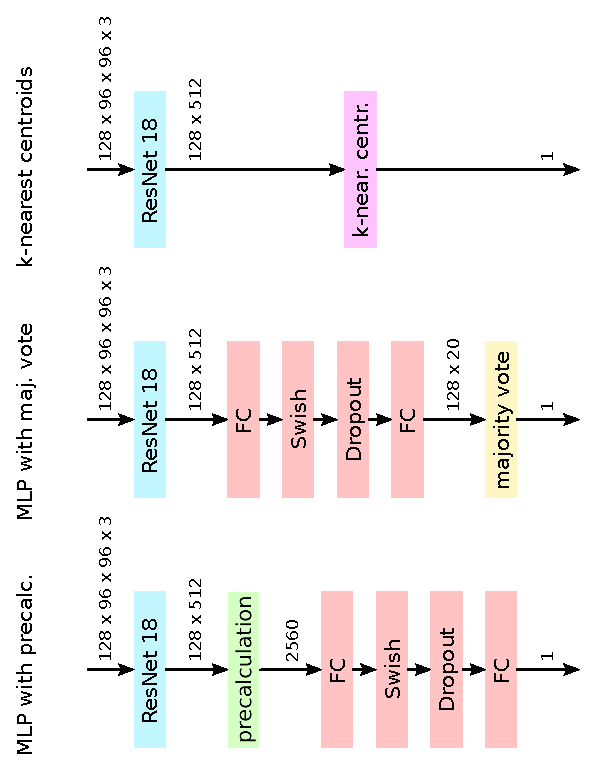
\includegraphics[width=0.8\linewidth]{../figures/approach1.eps} 
\end{center}
\caption{Overview of the different approaches based on an image classification network with typical implementation parameters}
\label{fig:approach1}
\end{figure} 
%

%%%%%%%%%%%%%%%%%%%%%%%%%%%%%%%%%%%%%%%%%%%%%%%%%%%%%%%%%%%%%%%%%%%%%%%%%%%%%%%%%
\subsection{Approach 2}
\label{sec:approach2}

The second approach uses the latent space of a variational autoencoder (VAE) as meta features. By pretraining the VAE on a large variety of images, similar images belonging to one dataset cluster together in latent space whereas dissimilar images from different datasets have a large (Euclidean) distance in latent space. When measuring both the mean and standard deviation of a batch of images in latent space for the test dataset and batches of images of the different training datasets, a two-sampled t-test is used to determine the ``nearest'' dataset. %Note that differing from the first approach the datasets to be pretrained on can be only a subset of the training datasets: If the VAE has been trained on a large variety of images (which may be contained in a single large dataset as ImageNet), it might be capable of reconstructing images from other (training) datasets as well, even it has never been trained on them. 

The VAE consists of a DenseNet 121 \cite{huang17} for the encoder and a PixelCNN++ \cite{salimans17} for the decoder, see Fig.~\ref{fig:approach2}. A fully connected layer maps the 196-dimensional latent space (i.e. the logits output of the DenseNet) to the 64x64x3-dimensional input of the PixelCNN++ network. Differing from the original DenseNet implementation, the first layer has been adjusted for the smaller image size to a 3x3 convolution with stride 1, no padding and no pooling after it. The VAE trained on seven different datasets (Caltech101, Colorectal Histology, DeepWeeds, EuroSAT, Food-101, ImageNet) whereas the last one has been resized to 64x64 pixel for faster calculation. These datasets have shown to yield a large variety of different images which are supposed to generalize well to other datasets.

%
\begin{figure}[htb]
\begin{center}
 	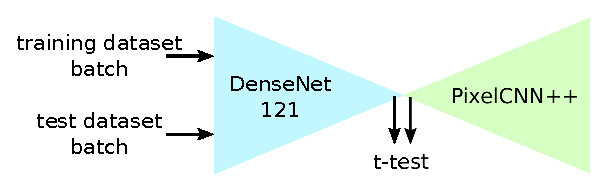
\includegraphics[width=0.8\linewidth]{../figures/approach2.eps} 
\end{center}
\caption{Overview of the VAE approach based on an image classification network for the encoder and a generative image network for the decoder.}
\label{fig:approach2}
\end{figure} 
% 


%%%%%%%%%%%%%%%%%%%%%%%%%%%%%%%%%%%%%%%%%%%%%%%%%%%%%%%%%%%%%%%%%%%%%%%%%%%%%%%%%
\subsection{Comparison of the two approaches}
\label{sec:comparison}

While the two approaches of section~\ref{sec:approach1} and~\ref{sec:approach2} are conceptually similar as they first learn a suitable embedding and then classify different datasets based on the information from the embedding, they have also some subtle differences:

\textbf{Number of parameters}: Both approaches are very small in terms of model parameters compared to current state-of-the-art image classification networks: Whereas a Resnet18 with the subsequent MLP with precalculation has around 12M parameters, the VAE has only around 7m parameters.

\textbf{Pretraining}: Both models can be pretrained well on a single dataset if it contains a large enough variety of images (e.g. ImageNet). Still, being a well-proven architecture a ResNet18 is probably even easier to train than a VAE. Moreover, there are mutliple sources with well pretrained Resnet18 models, making manual pretraining obsolete.

\textbf{Adding more training datasets}: Unless the additional training datasets differ significantly from the ones used for pretraining, both the Resnet18 of the first approach and the VAE of the second approach can be kept as-is. However, the first approach requires pretraining of the MLP from scratch whenever a training dataset is added.

\textbf{Dependence on training datasets during test time}: Because the first approach encodes the relation between different training datasets in the MLP, it requires only test data during test time. On the contrary, the second approach compares a batch from the test dataset with batches from all training datasets during test time using a two-sample t-test. Thus it needs access to the entire training datasets or at least the latent representation (mean and standard deviation) of a few selected batches of every training dataset during test time. 

\textbf{Dataset class classification}: Whereas the first approach is restricted to dataset classification, the second approach also allows for a more fine-grained classification: By comparing a batch of the test dataset to batches sampled from the same class of a training dataset, one can find not only the most similar dataset but also the most similar class of a dataset.

%%%%%%%%%%%%%%%%%%%%%%%%%%%%%%%%%%%%%%%%%%%%%%%%%%%%%%%%%%%%%%%%%%%%%%%%%%%%%%%%%
\subsection{Experiments}
\label{sec:experiments}

BOHB~\cite{falkner18} is used for the a priori calculation of optimized configurations $\theta^*(t_j)$ for different training datasets $t_j$. Every configuration consists of a pretrained network (either trained on ImageNet or CIFAR-100) and the following hyperparameters (if applicable):
%
\begin{itemize}
\item Optimizer: ADAM or SGD (with Nesterov momentum 0.9 and weight decay 1e-6)
\item Train batch size: 16/32/64/128
\item Learning rate: 1e-5 - 0.5
\item Dropout 0.01 - 0.99
\end{itemize}
%
An overview of the used datasets and models is given in Fig.~\ref{fig:dataset_results} and Fig.~\ref{fig:rank_results}. The two figures show the best classification accuracy in terms of ALC of the different models on the different datasets, both from a model-based perspective and a dataset-based perspective. The hyperparameters for every combination of dataset and model are optimized through 10 BOHB runs. Note that not all datasets listed in Tab.~\ref{table:datasets} appear in Fig.~\ref{fig:dataset_results}. Some are used as test datasets whereas others (especially video datasets) are too large to be processed efficiently with the given resources.

\begin{figure}[htb]
\begin{center}
 	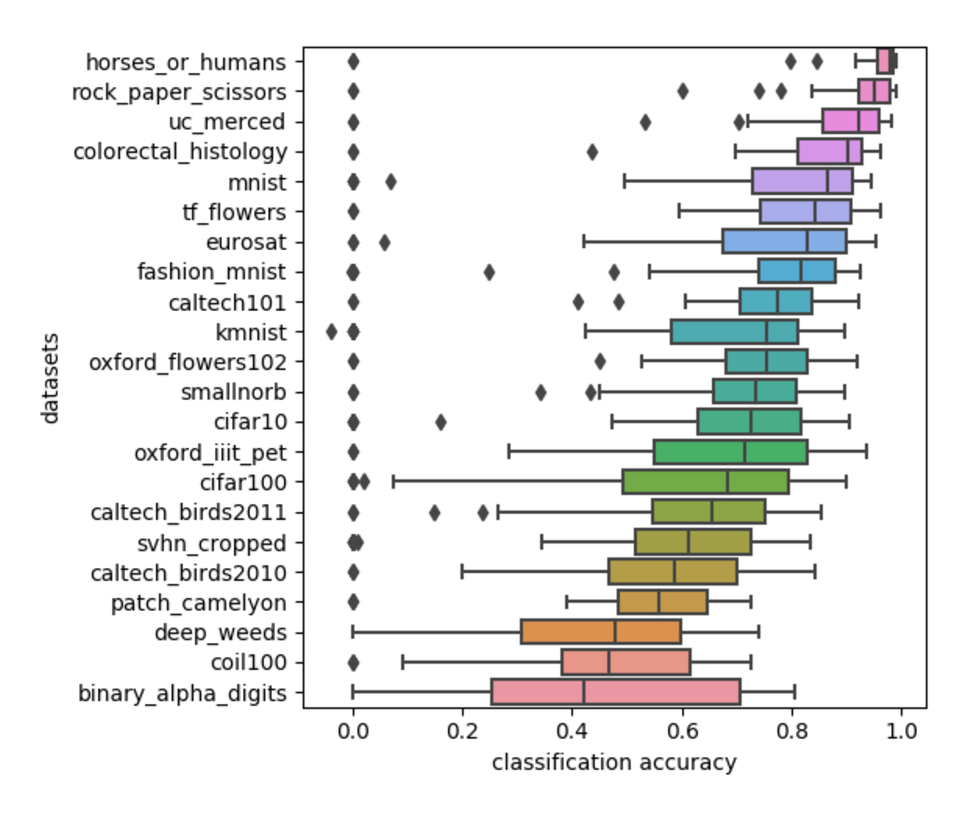
\includegraphics[width=0.85\linewidth]{../figures/dataset_results.eps} 
\end{center}
\caption{ALC of the different models across all datasets, sorted by dataset}
\label{fig:dataset_results}
\end{figure} 

\begin{figure}[htb]
\begin{center}
 	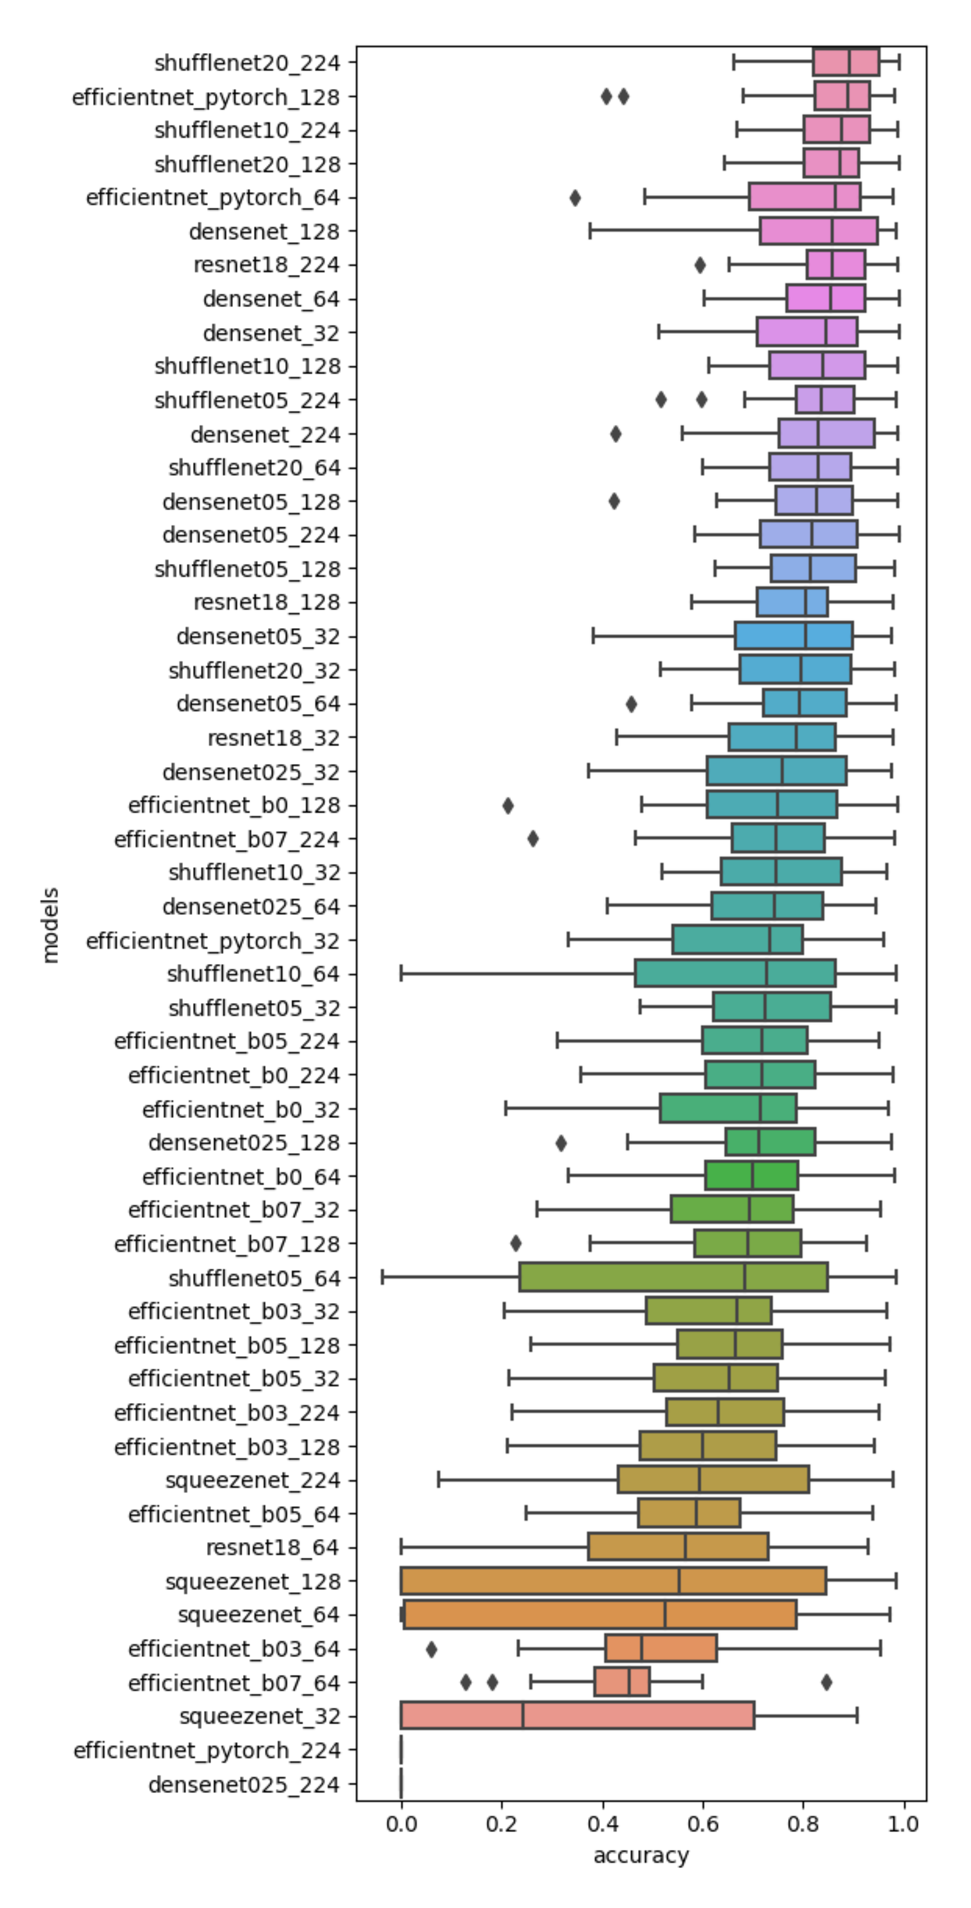
\includegraphics[width=0.85\linewidth]{../figures/accuracy_results.eps} 
\end{center}
\caption{ALC of the different models across all datasets, sorted by model}
\label{fig:rank_results}
\end{figure} 

In addition, multiple optimization runs find an optimal meta feature vector and a reasonable distance measure while keeping the configuration space $\Theta$ small: Being reasonably small and fast, a ResNet18 network pretrained on ImageNet serves as basis to generate the meta feature vector $\mathbf{m}(t_j)$. However, using the output of the second last layer yields consistently better results than the last output and is therefore chosen.

The following parameters have been optimized for the different approaches using BOHB: 

MLP:
\begin{itemize}
\item Train batch size: 1/2/4/8/16/32/64/128/256/512/1024
\item Neurons per layer: 16/32/64/128/256/512/1024
\item Learning rate: 1e-5 - 1e-2
\item Dropout rate: 0 - 0.8
\end{itemize}

MLP with precalculation:
%
\begin{itemize}
\item Train batch size: 1/2/4/8/16/32/64/128/256/512/1024
\item Neurons per layer: 16/32/64/128/256/512/1024
\item Learning rate: 1e-5 - 1e-2
\item Dropout rate: 0 - 0.8
\item p-quantile: 0 - 0.4
\item (Do not) use mean, median, standard deviation, variance, skewness, kurtosis
\end{itemize}
%

%\begin{figure}[!ht]
   %\begin{minipage}{\linewidth}
   %\centering
   %\includegraphics[width=.45\linewidth]{../figures/Chucky.eps}
   %\includegraphics[width=.45\linewidth]{../figures/Decal.eps}\\
	 %\includegraphics[width=.45\linewidth]{../figures/Hammer.eps}
   %\includegraphics[width=.45\linewidth]{../figures/Munster.eps}\\
	 %\includegraphics[width=.45\linewidth]{../figures/Pedro.eps}
   %\includegraphics[width=.45\linewidth]{../figures/Kraut.eps}\\
   %\includegraphics[width=.45\linewidth]{../figures/Katze.eps}
   %\includegraphics[width=.45\linewidth]{../figures/Kreatur.eps}
   %\caption{Final classification results}
   %\label{fig:results}
	 %\end{minipage}
%\end{figure}

%\begin{figure}[!ht]
   %\begin{minipage}{\linewidth}
   %\centering
   %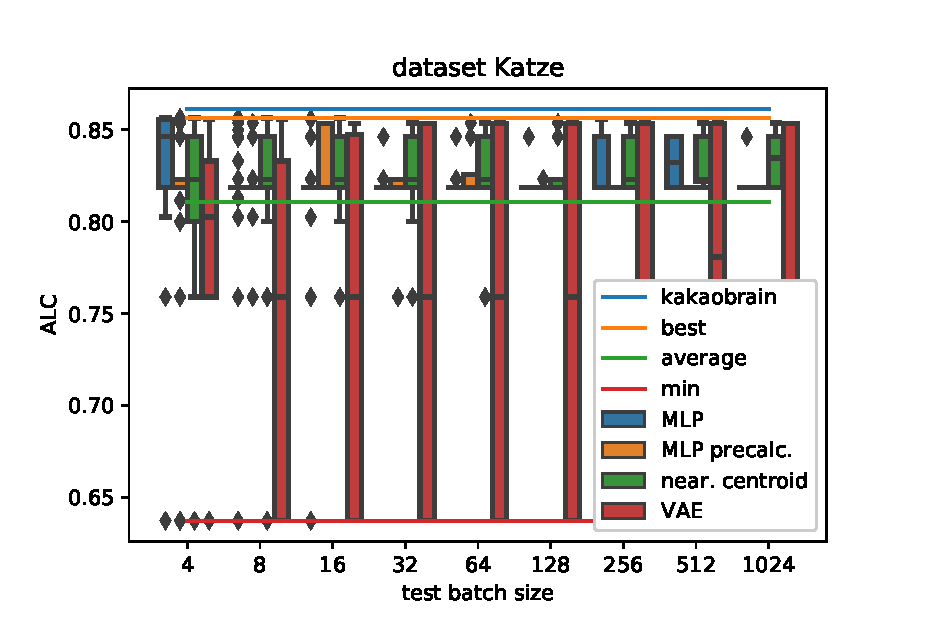
\includegraphics[width=.9\linewidth]{../figures/10.eps}
   %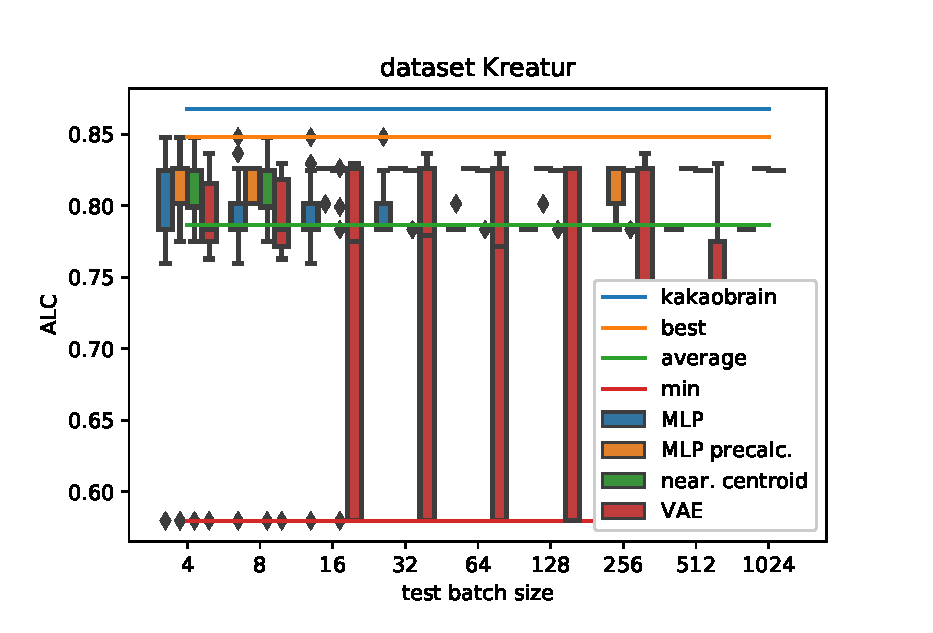
\includegraphics[width=.9\linewidth]{../figures/11.eps}
	 %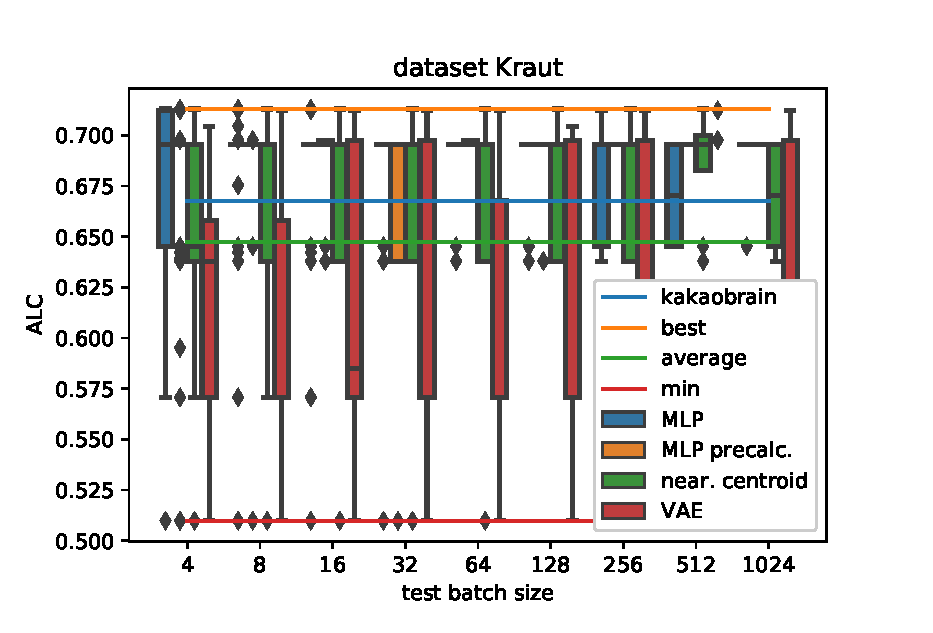
\includegraphics[width=.9\linewidth]{../figures/12.eps}
   %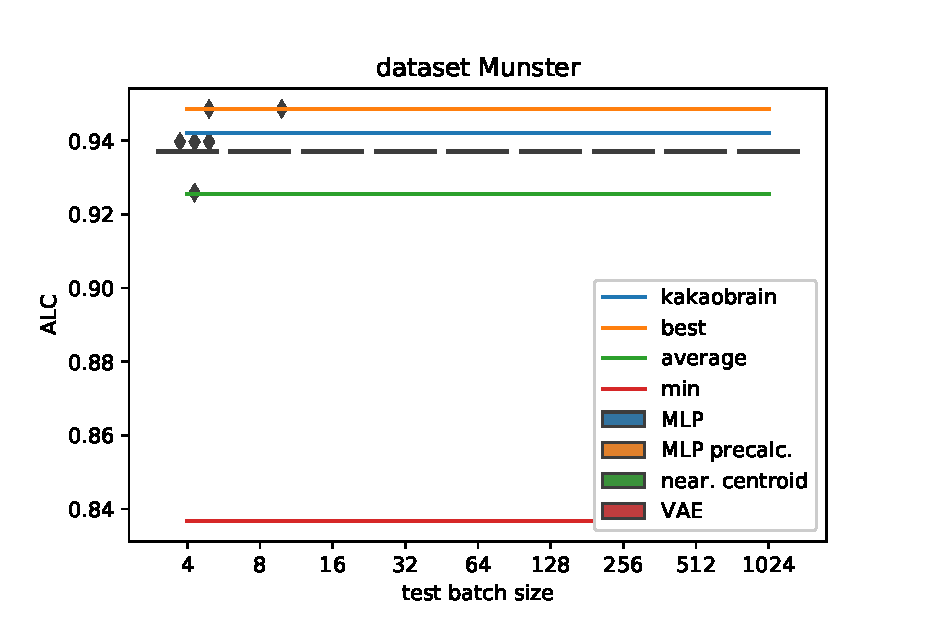
\includegraphics[width=.9\linewidth]{../figures/13.eps}
	 %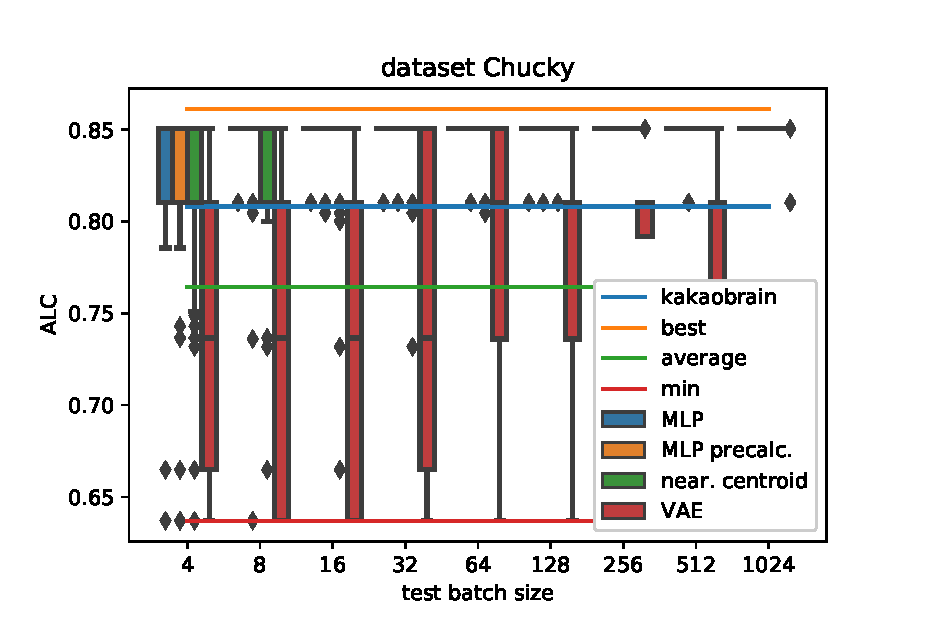
\includegraphics[width=.9\linewidth]{../figures/14.eps}
   %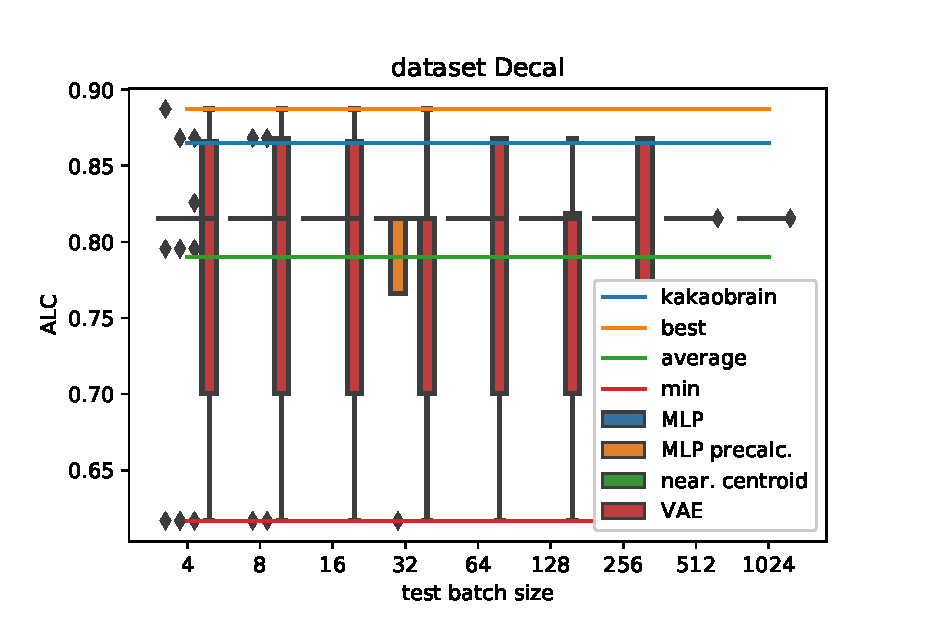
\includegraphics[width=.9\linewidth]{../figures/15.eps}
   %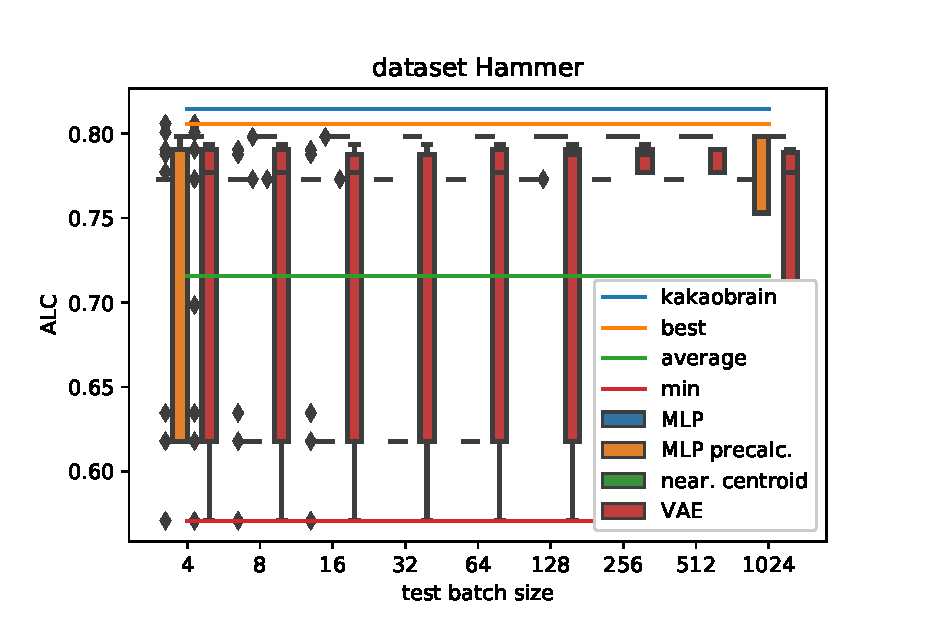
\includegraphics[width=.9\linewidth]{../figures/16.eps}
   %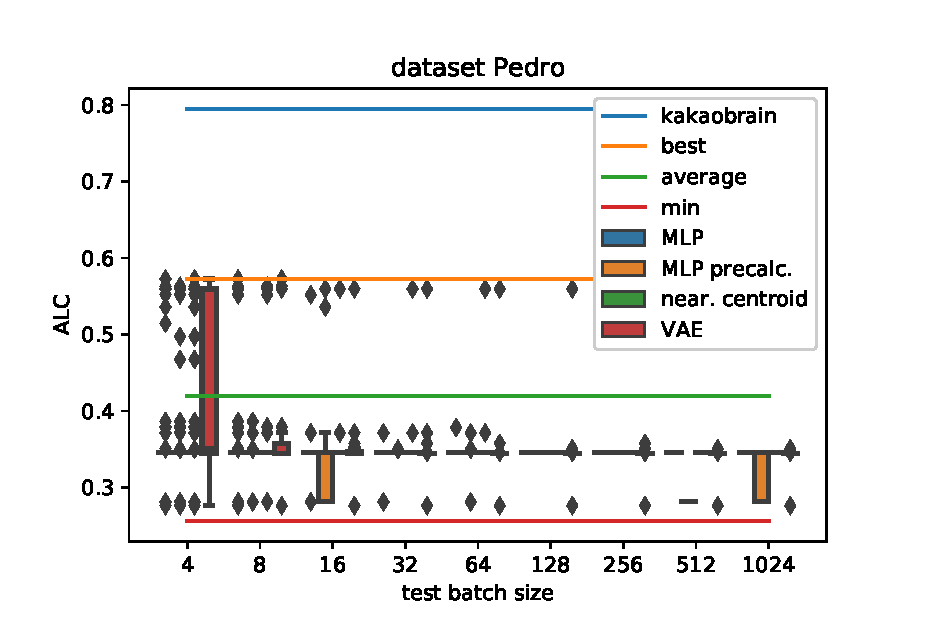
\includegraphics[width=.9\linewidth]{../figures/17.eps}
   %\caption{Final classification results}
   %\label{fig:results}
	 %\end{minipage}
%\end{figure}

%
\begin{figure}[H]
\begin{center}
 	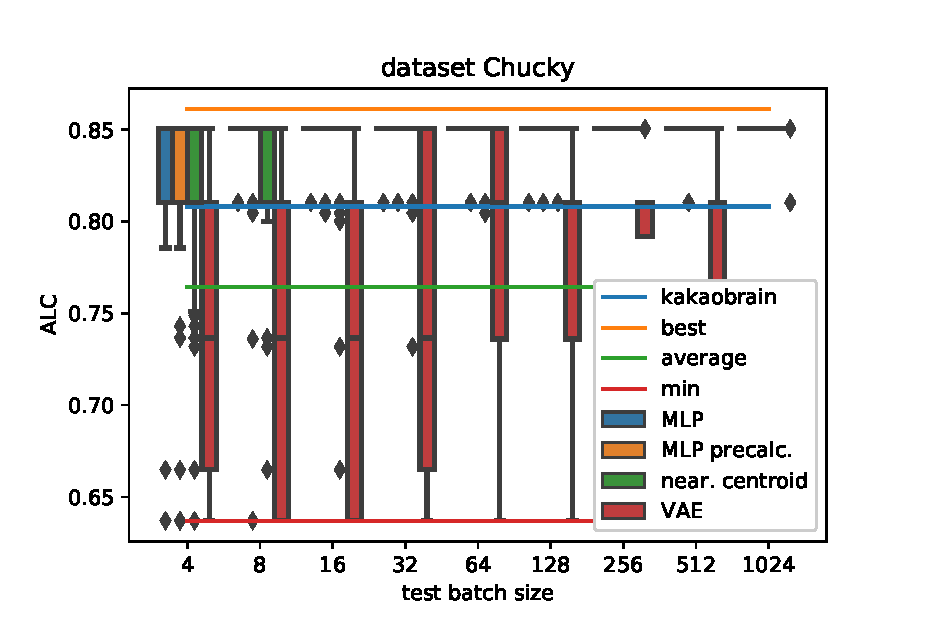
\includegraphics[width=0.99\linewidth]{../figures/14.eps} 
\end{center}
\caption{Test ALC for the different approaches for dataset Chucky}
\label{fig:14}
\end{figure} 
%
\begin{figure}[H]
\begin{center}
 	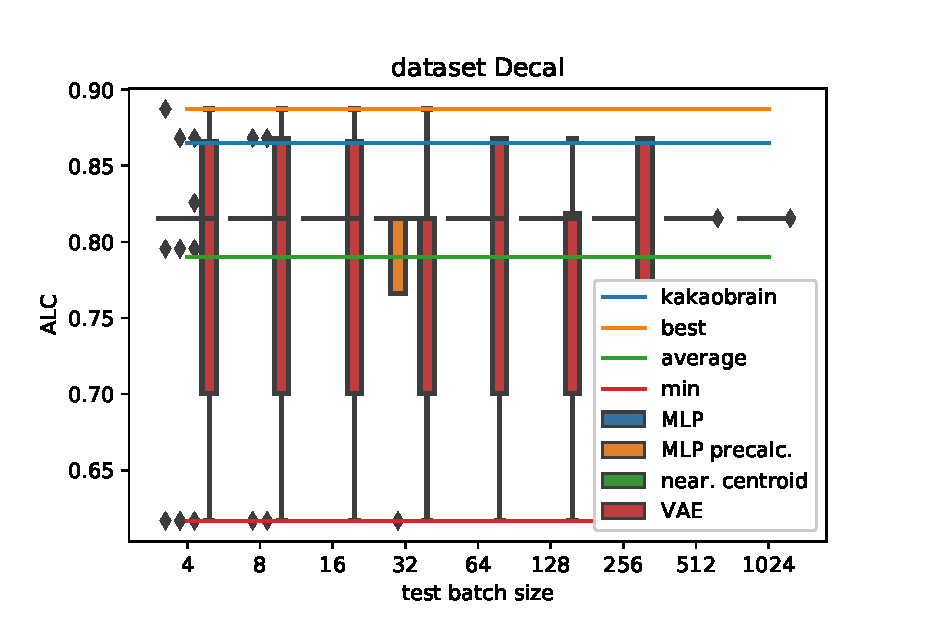
\includegraphics[width=0.99\linewidth]{../figures/15.eps} 
\end{center}
\caption{Test ALC for the different approaches for dataset Decal}
\label{fig:15}
\end{figure} 
%
\begin{figure}[H]
\begin{center}
 	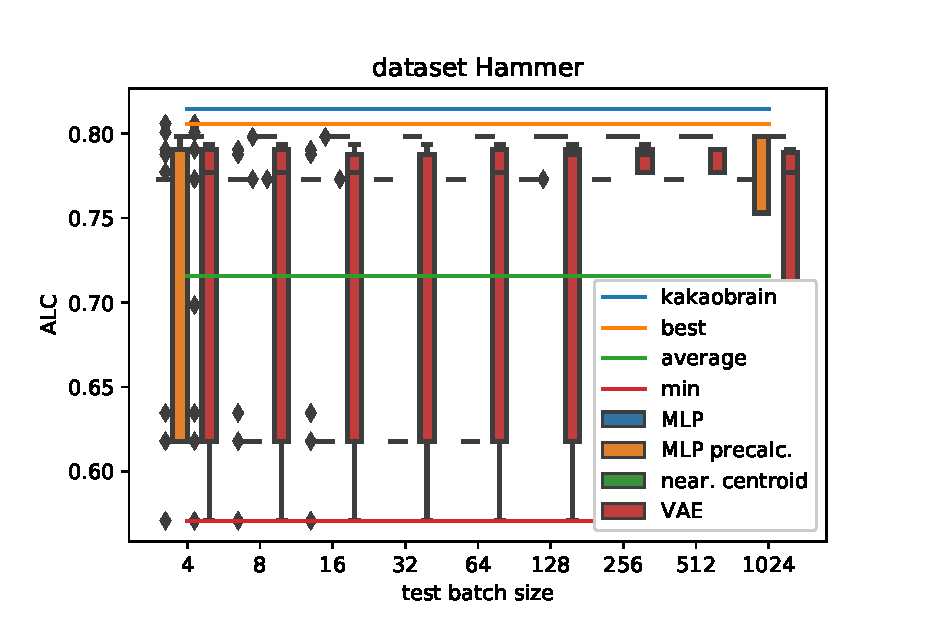
\includegraphics[width=0.99\linewidth]{../figures/16.eps} 
\end{center}
\caption{Test ALC for the different approaches for dataset Hammer}
\label{fig:16}
\end{figure} 
%
\begin{figure}[H]
\begin{center}
 	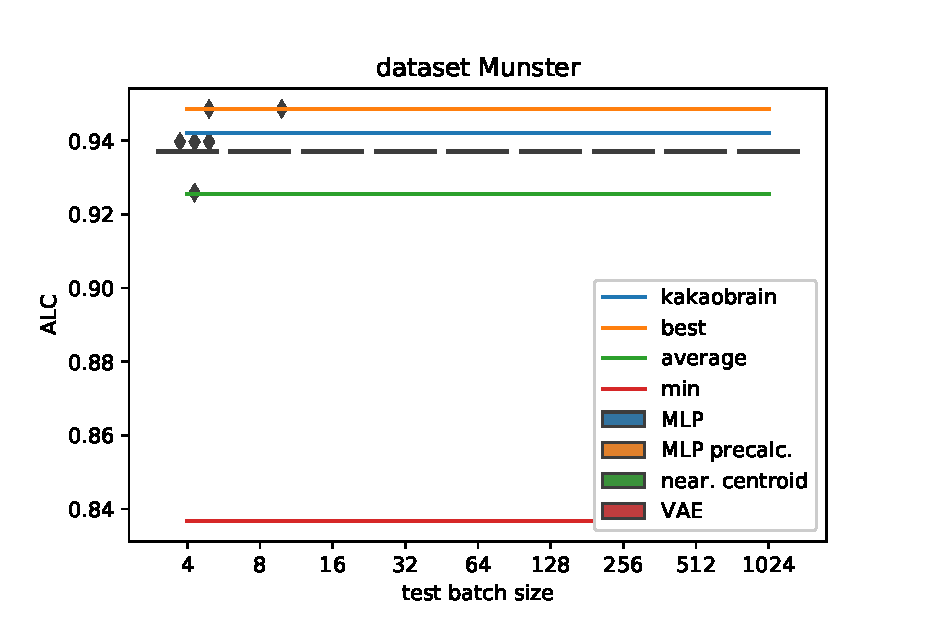
\includegraphics[width=0.99\linewidth]{../figures/13.eps} 
\end{center}
\caption{Test ALC for the different approaches for dataset Munster}
\label{fig:13}
\end{figure} 
%
\begin{figure}[H]
\begin{center}
 	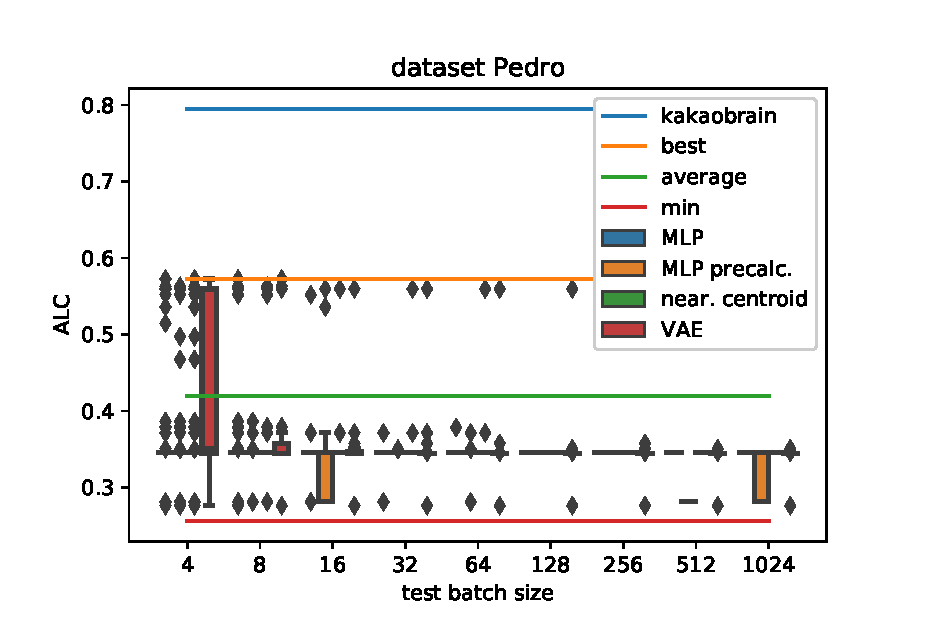
\includegraphics[width=0.99\linewidth]{../figures/17.eps} 
\end{center}
\caption{Test ALC for the different approaches for dataset Pedro}
\label{fig:17}
\end{figure} 
\begin{figure}[H]
\begin{center}
 	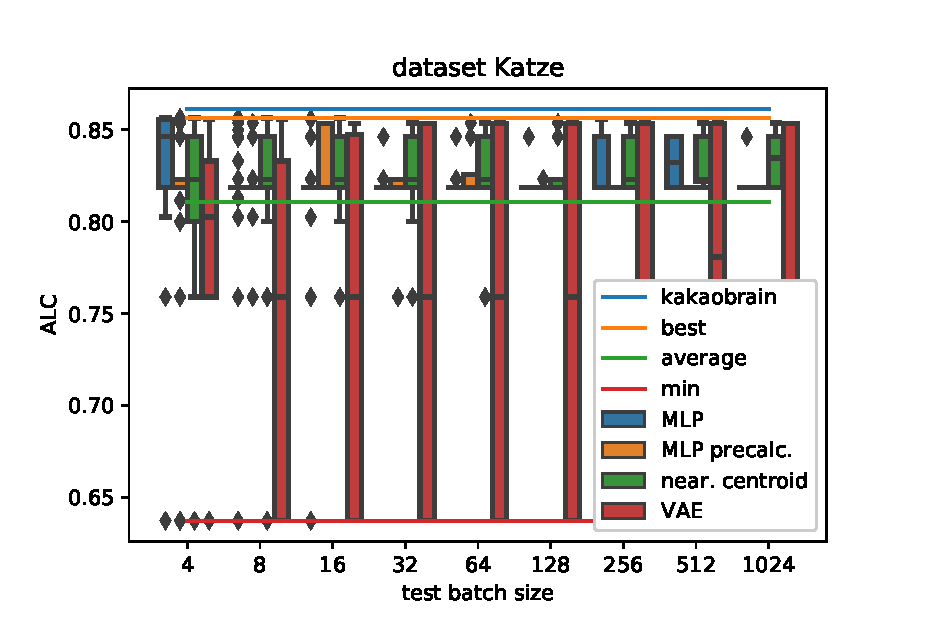
\includegraphics[width=0.99\linewidth]{../figures/10.eps} 
\end{center}
\caption{Test ALC for the different approaches for dataset Katze}
\label{fig:10}
\end{figure} 
%
\begin{figure}[H]
\begin{center}
 	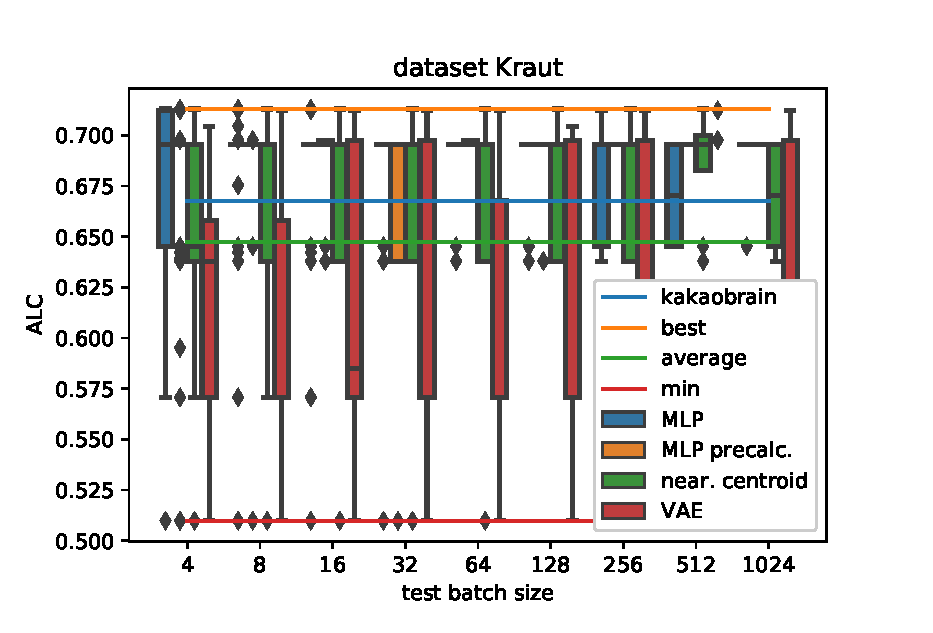
\includegraphics[width=0.99\linewidth]{../figures/12.eps} 
\end{center}
\caption{Test ALC for the different approaches for dataset Kraut}
\label{fig:12}
\end{figure} 
%
\begin{figure}[H]
\begin{center}
 	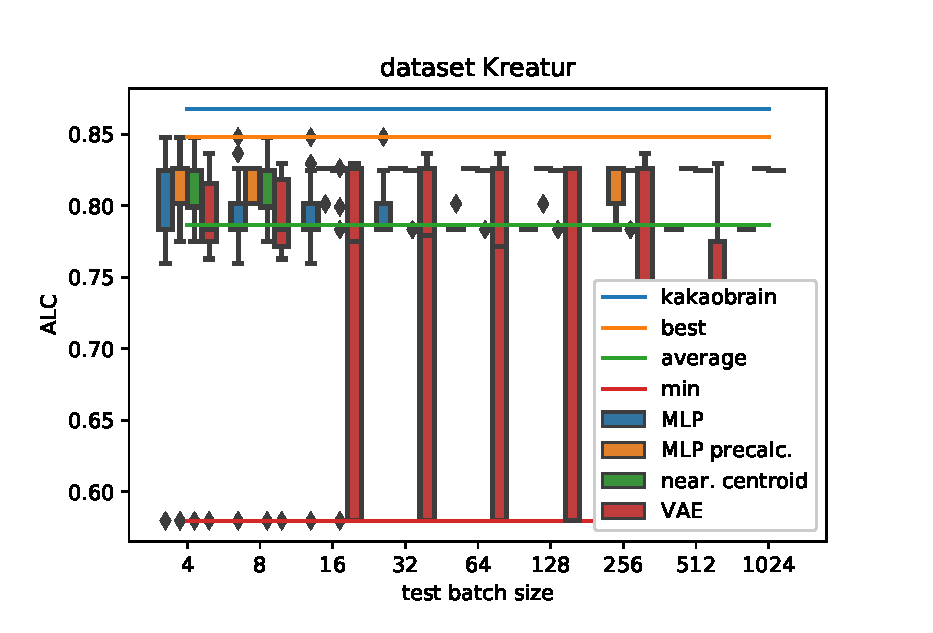
\includegraphics[width=0.99\linewidth]{../figures/11.eps} 
\end{center}
\caption{Test ALC for the different approaches for dataset Kreatur}
\label{fig:11}
\end{figure} 

Final results of the different approaches are shown in Fig.~\ref{fig:14}-Fig.~\ref{fig:11}. The eight plots correspond to the eight test datasets (Chucky, Decal, Hammer, Munster, Pedro, Kraut, Katze, Kreatur). Every plot shows the test ALC according to Eq.~(\ref{eq:ALC}) over the test batch size of the classification networks of section~\ref{sec:approach1} and~\ref{sec:approach2}. The different thick solid lines correspond to:
\begin{itemize}
\item \textbf{kakaobrain}: ALC results from the winning AutoCV and AutoCV2 team kakaobrain \cite{kakaobrain}.
\item \textbf{best}: Best ALC of all incumbents of the training datasets evaluated on the test dataset
\item \textbf{avg}: Average ALC of all incumbents of the training datasets evaluated on the test dataset
\item \textbf{min}: Minimum ALC of all incumbents of the training datasets evaluated on the test dataset
\end{itemize}
Thus, a plot ideally has the following appearance: Kakaobrain has the highest ALC as we do not expect to perform better than a team of computer vision professionals, followed by the different ALCs of the incumbents of the training datasets evaluated on the test dataset.

There are several effects why the plots in Fig.~\ref{fig:results} differ from the ideal plot described before: 

Sometimes an incumbent yields a better ALC than kakaobrain. A possible reason is the different ALC calculation: Due to heavily varying execution times on the cluster (up to a factor of 10) we did not measure the real ALC. Rather, the execution time of an individual forward and backward pass for every model for images/videos of different input shapes has been measured on a reference system and been stored in a lookup table. The lookup table is then used on the cluster to estimate the ALC based on the number of batches, the number of samples per batch and the average shape of the images/videos of the dataset. This procedure allows one to be independent of the cluster execution time while having a good approximation of the true ALC but may overestimate the true ALC.

For some datasets (e.g. Munster) the ALC varies very little across different test batch sizes. Although this is the preferred case (the output of the meta classifier is ideally independent of the batch size), the effect is usually caused by the test dataset being similar to one of the training datasets. Then a well-trained meta classifier always correctly classifies the test dataset being most similar to the (identical) training dataset.

Choosing an optimal test batch size is crucial during test time. When being too small, the meta classifier may produce noisy (and thus possibly incorrect) predictions. When being too large, more samples than necessary are processed. This leads to computational overhead. 

%%%%%%%%%%%%%%%%%%%%%%%%%%%%%%%%%%%%%%%%%%%%%%%%%%%%%%%%%%%%%%%%%%%%%%%%%%%%%%%%%
\section{Discussion}
\label{sec:discussion}

Results of the AutoCV2 challenge have shown that it is not sufficient for any non-CV expert to rely on a single video classification network. Thus the meta learning approach with a portfolio of different classification networks has been developed. Although being effective, finding incumbent configurations for more than 20 datasets for more than 50 models is time-consuming and took around two weeks using 40 GPUs. In addition, Fig.~\ref{fig:rank_results} indicates that it is sufficient to use a much smaller portfolio of e.g. only the ten models with the average best performance. A small experiment leads to the result in Fig.~\ref{fig:portfolio_performance} where the optimized averaged best performance across all datasets is plotted over the model portfolio size.  With averaged best performance we are referring to the best performance of all the models in the portfolio for every dataset, averaged over all datasets. The plot indicates that is is sufficient to use as few as five carefully selected models to achieve an almost similar performance as with all 52 models.
%
\begin{figure}[htb]
\begin{center}
 	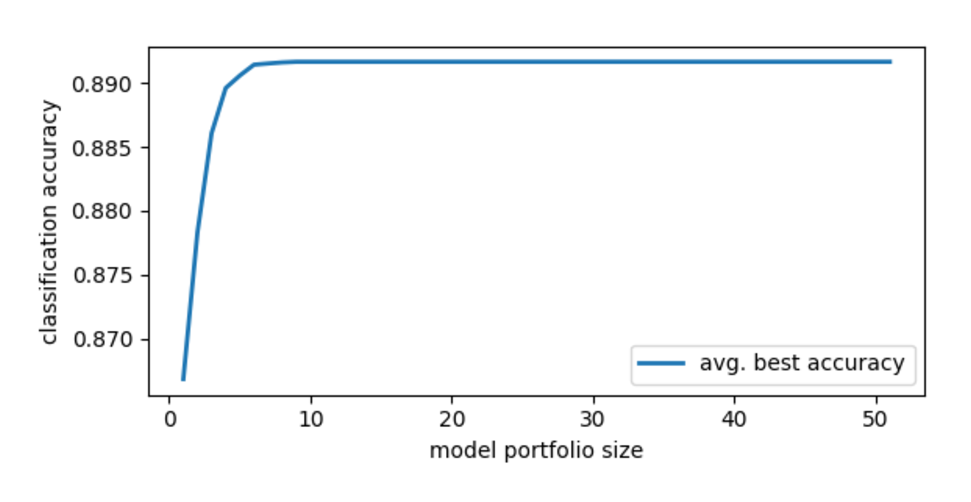
\includegraphics[width=0.85\linewidth]{../figures/portfolio_performance.eps} 
\end{center}
\caption{Averaged best performance of a reduced model portfolio across all datasets}
\label{fig:portfolio_performance}
\end{figure} 
%

A more substantial critic concerns the format of the AutoDL challenge: By using the ALC score (more specifically: the logarithmic time scale), submissions with very good results from the beginning on are favored. Albeit this is desired by the organizers, it became more an engineering problem than an interesting research challenge to optimize the data loading pipeline, strip state-of-the-art models to the bare minimum and evaluate how long they produce reasonable results. This is backed by the observation that the winners of both the AutoCV and AutoCV2 challenge used rather simple base models (Resnet9 and Resnet18) and their superior performance is the result of the combination of many small, existing tweaks instead of a completely new approach.

Using the wall clock time to calculate the ALC score was an major issue for reproducibility and portability across multiple systems. As such the final results for the AutoCV2 challenge were calculated as the average of three individual runs. The wall clock time issues was worst on the computing cluster in Freiburg. The combination of a high data throughput when classifying image/video datasets and the use of HDDs led to a huge variance in execution speed - sometimes up to a factor of 10. Thus the workaround with the execution time lookup table described in Sec.~\ref{sec:experiments} has been chosen.

In the end we were suprised how conceptually simple our approach was. Distinguishing different datasets seems to be an easier problem than distinguishing different classes within a dataset. As such the simplest approach (Resnet18 +  k-nearest centroids) provides surprisingly good results. However, this simplicity comes with the drawback of a large computational load when computing the incumbents for the different training datasets.

%%%%%%%%%%%%%%%%%%%%%%%%%%%%%%%%%%%%%%%%%%%%%%%%%%%%%%%%%%%%%%%%%%%%%%%%%%%%%%%%%
\section{Summary and Outlook}
\label{sec:summary}

We present two conceptually different methods for quick generalization of a pretrained network to new datasets in the context of the AutoCV2 and AutoDL challenge. Whereas the first method relies on transfer learning (i.e. pretraining a model and then fine tuning it on the new dataset), the second approach considers a portfolio of different models and selects the model that performed best on a dataset that is most similar to the new dataset.
Thus focus shifts from finding a single state-of-the-art model working well on a variety of different datasets to measuring the similarity between two datasets and selecting the one that is most similar - the latter being much easier to implement for anyone who is not an expert in video classification. 

There are several directions for future work: The first one considers redundancy in the datasets. It is shown in the discussion chapter how the used models are highly redundant and the model portfolio can be reduced by a factor of 10 without severe performance loss. It is unknown (but suspected) if the same applies for the datasets, i.e. if training the models on a small but carefully selected set of datasets leads to the same generalization performance. 

The second tackles the choice of meta features. All used meta features are located in the embedding space of either a image classification network or a VAE. It is an open question if a different choice of meta features yields substantially better results.

Furthermore, the VAE approach of Sec.~\ref{sec:approach2} is a promising idea for future expansions. It is an open question if more advanced classification methods using the latent space representation (e.g. neural networks) lead to better classification results than a two-sample t-test. 

\bibliography{../bib/autodl}
\bibliographystyle{icml2018}

\end{document}


% This document was modified from the file originally made available by
% Pat Langley and Andrea Danyluk for ICML-2K. This version was created
% by Iain Murray in 2018. It was modified from a version from Dan Roy in
% 2017, which was based on a version from Lise Getoor and Tobias
% Scheffer, which was slightly modified from the 2010 version by
% Thorsten Joachims & Johannes Fuernkranz, slightly modified from the
% 2009 version by Kiri Wagstaff and Sam Roweis's 2008 version, which is
% slightly modified from Prasad Tadepalli's 2007 version which is a
% lightly changed version of the previous year's version by Andrew
% Moore, which was in turn edited from those of Kristian Kersting and
% Codrina Lauth. Alex Smola contributed to the algorithmic style files.
